\documentclass{article}
\usepackage[a4paper, hmargin={2.8cm, 2.8cm}, vmargin={2.5cm, 2.5cm}]{geometry}
%%%%%%%%%%%%%%%%%%%%%%%%%%%%%%%%%%%%%%%%%%%%%%%%%%%%%%%%%%%%%%%%%%%%%%%%%%%%%%%%

%%%%%%%%%%%%%%%%%%%%%%%%%%%%%%%%%%%%%%%%%%%%%%%%%%%%%%%%%%%%%%%%%%%%%%%%%%%%%%%%
\usepackage[utf8]{inputenc}
\usepackage[T1]{fontenc}
%%%%%%%%%%%%%%%%%%%%%%%%%%%%%%%%%%%%%%%%%%%%%%%%%%%%%%%%%%%%%%%%%%%%%%%%%%%%%%%%


%%%%%%%%%%%%%%%%%%%%%%%%%%%%%%%%%%%%%%%%%%%%%%%%%%%%%%%%%%%%%%%%%%%%%%%%%%%%%%%%
\usepackage{mathtools}
\usepackage{amsthm}
\usepackage{amssymb}
\usepackage{csvsimple}
\usepackage{subcaption}
\usepackage{url}
\usepackage{tikz}
\usepackage{pgfplots}
%%%%%%%%%%%%%%%%%%%%%%%%%%%%%%%%%%%%%%%%%%%%%%%%%%%%%%%%%%%%%%%%%%%%%%%%%%%%%%%%


%%%%%%%%%%%%%%%%%%%%%%%%%%%%%%%%%%%%%%%%%%%%%%%%%%%%%%%%%%%%%%%%%%%%%%%%%%%%%%%%
\usepackage{fancyhdr}
\usepackage{graphicx}
\usepackage{parskip}
\usepackage{listings}
\usepackage{enumitem}
\usepackage{titlesec}
\usepackage[lastpage,user]{zref}
\usepackage{caption}
\usepackage{scrextend}
\usepackage[outputdir=./.latex-out]{minted} % TODO slet hvis du ikke bruger minted
\usepackage{listings}
\usepackage{blindtext}
%%%%%%%%%%%%%%%%%%%%%%%%%%%%%%%%%%%%%%%%%%%%%%%%%%%%%%%%%%%%%%%%%%%%%%%%%%%%%%%%
\newcommand{\python}[1] {
  \mintinline{python}{#1}
}
\newcommand{\tex}[1] {
  \mintinline{latex}{#1}
}

\pagestyle{fancy}
%%%%%%%%%%%%%%%%%%%%%%%%%%%%%%%%%%%%%%%%%%%%%%%%%%%%%%%%%%%%%%%%%%%%%%%%%%%%%%%%
%%%%%%%%%%%%%%%%%%%%%%%%%%%%%%%%%%%%%%%%%%%%%%%%%%%%%%%%%%%%%%%%%%%%%%%%%%%%%%%%
\lhead{\LaTeX webinar} % TODO indsæt venstre sidehoved
\rhead{Study Now} % TODO indsæt højre sidehoved
\cfoot{\thepage\ of \zpageref{LastPage}}
\newtheorem*{prp}{Propostion}
\setlist{nolistsep}
%%%%%%%%%%%%%%%%%%%%%%%%%%%%%%%%%%%%%%%%%%%%%%%%%%%%%%%%%%%%%%%%%%%%%%%%%%%%

%%%%%%%%%%%%%%%%%%%%%%%%%%%%%%%%%%%%%%%%%%%%%%%%%%%%%%%%%%%%%%%%%%%%%%%%%%%%
\title{
  \vspace{13em}
  \large{Study Now} \\
  \Large{\LaTeX webinar} \\
}

\author{
  Benjamin Rotendahl --- Benjamin@Rotendahl.dk
}

\date{
  \vspace{22em}
  \today
}

\begin{document}
\maketitle		% Forside
\thispagestyle{empty}
\newpage

\section{Introduktion}
 Dette dokument fungerer som et \emph{cheatsheet}. Det gennemgår de forskellige
 former for opsætning og funktioner i \LaTeX. Når du selv sidder og skriver, kan
 du enten bruge den færdige PDF som opslagsværk, eller kigge på kildekoden.
 Husk, at du selv kan udvide dokumentet med yderligere sektioner, hvis du finder
 nogle seje funktioner i din videre færd med \LaTeX{}.
Har du lyst til at se hele videokurset så gå ind på:
\url{https://ida.studynow.dk/courses/take/latex-for-begyndere/surveys/26409734-tre-sporgsmal-for-vi-starter}



\section{Leg}\label{sec:leg}
 Hej med jer!
 \subsection{Leg med matematik}
   Vi er nu i sektion~\ref{sec:leg}. Vi har \(x_k\) at at \(x + 2 = 4\)
   Dette dokument fungerer som et \emph{cheatsheet}. Det gennemgår de forskellige
   former for opsætning og funktioner i \LaTeX. Når du selv sidder og skriver, kan
   du enten bruge den færdige PDF som opslagsværk, eller kigge på kildekoden.
   Husk, at du selv kan udvide dokumentet med yderligere sektioner, hvis du finder
   nogle seje funktioner i din videre færd med \LaTeX{}.
   Har du lyst til at se hele videokurset så gå ind på:
   \begin{equation}\label{eq:leg}
     2 \tau = \pi = \gamma
   \end{equation}

Dette dokument fungerer som et \emph{cheatsheet}. Det gennemgår de forskellige
former for opsætning og funktioner i \LaTeX. Når du selv sidder og skriver, kan
du enten bruge den færdige PDF som opslagsværk, eller kigge på kildekoden.
Husk, at du selv kan udvide dokumentet med yderligere sektioner, hvis du finder
nogle seje funktioner i din videre færd med \LaTeX{}.
Har du lyst til at se hele videokurset så gå ind på:

\begin{flalign*}
  f(x,y)                        & = x^2 + y^3 \\
  \frac{\partial f}{\partial x} & = 2x + 3y^2
\end{flalign*}

\section{sub and superscripts}
 \[
   \int{i=1}^{n} x_i
 \]
\section{Matematik i \LaTeX}
 Latex' største styrke er dens evne til at formatere matematisk notation.
 For at skrive matematik skal man fortælle compileren, at den skal gå i
 \emph{math mode} for så at kunne skrive matematik specifikke kommandoer.
 Prøver man f.eks. at skrive \tex{\pi} uden at være i math mode, fejler den.
 Man kan som nævnt gå i inline math mode ved at skrive \tex{\(\pi\)}, som giver
 \(\pi\). Der findes også miljøer, som sætter en i math mode, f.eks. \tex{\equation}
 miløjet. Det går det også muligt at lave referencer til sine formler, f.eks.
 viser ligningen \eqref{dot} formlen for prikproduktet af to vectorer.
 \begin{equation}\label{dot}
   \vec{a} \cdot \vec{b} = \sum_{i=1}^{n} a_i b_i
 \end{equation}
 Koden, der producerer overstående, kan ses i ekspempel~\ref{lst:dot}
 \begin{listing}[!h]
   \begin{minted}[tabsize=1]{latex}
\begin{equation}\label{dot} % Label som kan bruges som reference
  \vec{a} \cdot \vec{b} = \sum_{i=1}^{n} a_i b_i
\end{equation}
\end{minted}
   \caption{Ligning for prikproduktet}\label{lst:dot}
 \end{listing}

Ønsker vi at have en flere trin i en udledning, kan vi bruge flalign-miløjet.
Der kan man have flere linjer, som bliver centreret efter placeringen af \tex{&}
symbolet.
\begin{flalign}
  f(x, y)                       & = 3x^2y + y^2 \\
  \frac{\partial f}{\partial x} & = 6xy         \\
  \frac{\partial f}{\partial y} & = 3x^2 + 2y
\end{flalign}
Koden, der skaber overstående, kan ses i listing~\ref{lst:diff}. Ønsker man at
fjerne tallene ude i højre side, kan det gøres ved at erstatte \tex{flaling} med
\tex{flaling*}.
\begin{listing}[!h]
\begin{minted}[tabsize=1]{latex}
\begin{flalign}
  f(x, y)                       & = 3x^2y + y^2 \\
  \frac{\partial f}{\partial x} & = 6xy         \\
  \frac{\partial f}{\partial y} & = 3x^2 + 2y
\end{flalign}
\end{minted}
\caption{Eksempel på formler centreret over flere linjer}\label{lst:diff}
\end{listing}

For at lave paranteser i sine formler skal man bare skrive som normalt, men
ønsker man, at de \(\begin{bmatrix} x & y & z \end{bmatrix}\) skalerer efter indholdet, så kræver det, at man skriver
\tex{\left ( x^2 \right )} rundt om. Typen af parenteser efter \tex{\left, \right}
kommandoen bestemmer,  hvordan det ser ud. Listing~\ref{lst:par} viser, hvordan følgende
er lavet.

\[
  1 + \tau = \left ( \frac{\pi}{2} \right ) + 1
\]

\section{matricer}
 \[
 \begin{bmatrix}
1 & 2 & 3 \\
4 & 5 & 6 \\
7 & 8 & 9
\end{bmatrix}
\]
fancy thing
\[
\begin{bmatrix}
1 & \dots & n \\
\vdots & 5 & 6 \\
7 & 8 & 9
\end{bmatrix}
\]

\section{Hvordan compiler man i latex}
 Det kan du se i figur~\ref{fig:comp}
 \begin{figure}[h]
   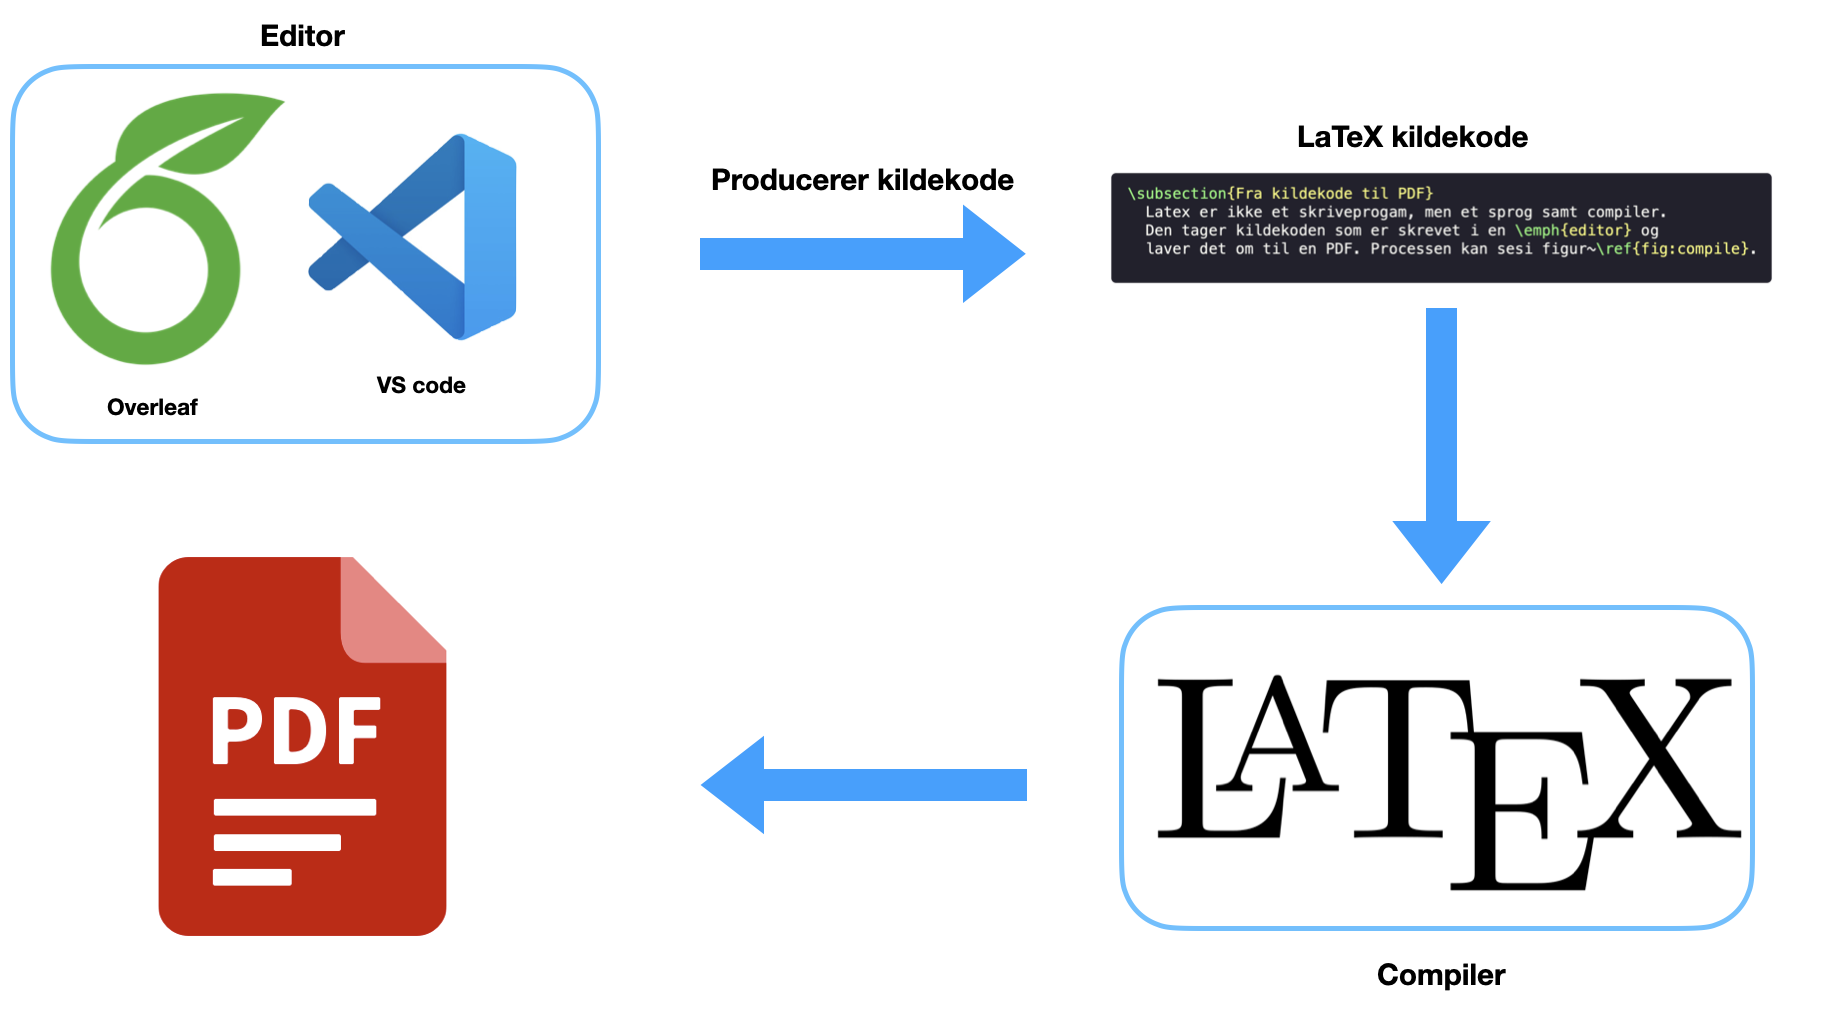
\includegraphics[width=0.8\linewidth]{assets/compile.png}
   \caption{Her er hvordan vi kompilerer}\label{fig:comp}
 \end{figure}




\end{document}


